%%%%%%%%%%%%%%%%%%%%%%%%%%%%%%%%%%%%%%%%%%%%%%%%%%%%%%%%%%%%%%%%%%%%%%%%%%%%%%
\chapter{Signal Processing Theory}
\label{cha:SignalProcessingTheory}

This chapter describes techniques of signal processing, which are required to receive and decode an FM broadcast radio signal.
The entire signal processing chain from the antenna, through the analog front-end, to the digital processing parts is explained.
However, the main focus is put on the digital signal processing part, since this is a major part of the practical implementation of this thesis.

%%%%%%%%%%%%%%%%%%%%%%%%%%%%%%%%%%%%%%%%%%%%%%%%%%%%%%%%%%%%%%%%%%%%%%%%%%%%%%
\section{Overview}
%TODO: this is copied from introduction:
%Evolution from AM to FM because of certain advantages, etc.\\
%Explain FM usage/existence nowadays (geographical; frequencies; devices; new %standard DAB, etc)

Wireless transmission systems usually transmit their signals over the air.
Various frequency bands and different types of modulation are being used for this purpose.
The choice of frequency, as well as the choice of the modulation type, have impacts on the transmission characteristics.
Depending on these choices, positive effects can be achieved in the amount of data that can be sent over the transmission channel, for example.
Another advantage is the ability to adapt the ongoing transmission to the changing characteristics of the channel.
This is especially useful for mobile receivers, since the signals' path is inherently changing over time there, which leads to challenging conditions for the receiver.
Additionally, varying signal strength, or multipath propagation may occur.
Multipath propagation is caused by reflections of the signal, which - for example - can occur on a house facade, or a large vehicle that is passing by.
The receiver then gets a signal, that is a summation of the direct path and the reflected path - a signal from multiple paths.
Besides that, environmental impacts, such as rain or fog have an effect on the transmission channel and thus the received signal.\\

Many more factors could be listed, and elaborations over the various modulation types fill entire books.
However, with all these different facts, there are things that they all have in common.
On the transmitter side, all these signals are transmitted in a band-limited, high frequency signal.
The band limitation needs to be given at the transmitting antenna, to minimize interference to other bands in the frequency spectrum.
The frequency needs to be high, to radiate the signal by an antenna.

On the receiver side, once the signal reaches the antenna of a receiver, there are further similarities.
The antenna signal needs to be amplified and filtered at first.
Both steps depend on the antenna characteristics, but usually the received signal is of relatively low power, and the antenna receives a wider range of frequencies than required.
The filter therefor selects the frequency area that is of interest.
Another reason for the filter is to avoid spectral replicas in the subsequent modulation, or down-conversion.
Here, the front-end often down-converts to a low intermediate frequency (IF), instead of directly going to baseband.
The intermediate frequency is then shifted down to baseband by a modulator later in the digital domain, which brings advantages in the downstream processing chain. %TODO check this or explain more which advantages (HF to BB directly --> i/q complex signal? ; HF to IF to BB --> real signal ) ??

These three steps - amplification, filtering and down-conversion to an IF - are often done in the analog domain, since digital circuits cannot work with such high frequencies.
After the analog signal is down-converted to baseband, it needs to be digitized.
This is done by an analog-digital-converter (ADC).

After the signal is processed to digital baseband, the received signal can finally be decoded to get the actual data content.
This decoding process depends on the respective modulation type that is used.\\

\noindent
The block diagram in Fig.\ref{fig:bd_dsp_overview} gives a high-level overview of a receiver structure.

\includepicture [1.0] [0] {High-level block diagram of a signal processing chain.} {bd_dsp_overview} {img/draw.io/bd_dsp_overview}

%%%%%%%%%%%%%%%%%%%%%%%%%%%%%%%%%%%%%%%%%%%%%%%%%%%%%%%%%%%%%%%%%%%%%%%%%%%%%%
\section{Receiver types}

Multiple different receiver architectures exist and are implemented in receivers.
Two common examples are explained in the following sections.

%%%%%%%%%%%%%%%%%%%%%%%%%%%%%%%%%%%%%%%%%%%%%%%%%%%%%%%%%%%%%%%%%%%%%%%%%%%%%%
\subsection{Superheterodyne Receiver}

The superheterodyne receiver is often referred to as \textit{superhet}, or \textit{super} in the literature.
The main characteristic of a superhet is, that it converts the radio-frequency (RF) antenna signal to an IF in a first stage, instead of going to baseband directly.\\

The IF is usually set to a fixed frequency, which results in the advantage, that the subsequent IF filter can be optimized, since it does not have to be adapted in frequency.
Therefore, a superhet receiver is able to select narrow band signals, even if the bands' surrounding frequencies are being used by other signals.
This is one of the superhets' main advantages.
A disadvantage is that the signal noise around the image frequency band is translated into the IF output band.
Thus, the filter requirements are relatively high, since they need to deliver a strong attenuation in order to suppress noise outside the desired band.

Fig.\ref{fig:bd_superhet} shows a block diagram of a superhet receiver.
The antenna signal first runs through a band selection filter.
It selects the desired frequency band and filters out any unwanted signals outside of this band.
A low-noise amplifier (LNA) may be used to boost the signal strenght.
The next step is the mixer, which is fed by a local oscillator (LO).
This shifts, or down-converts, the antenna signal down to the IF.
Afterwards, the IF signal is amplified and filtered again to remove the side-products of the mixer, namely the image replicas.
Thus, it is also called an image rejection filter.
The demodulator stage can now perform any further signal processing on the signal, until the required signal is retrieved \cite{PassosFábio2020AHSo}.\\

The depicted block diagram may represent an FM broadcast receiver, where an audio output is generated from the antenna input.

\includepicture [1.0] [0] {Block design of a superhetorodyne receiver \cite[Fig.2.1]{PassosFábio2020AHSo}} {bd_superhet} {img/draw.io/superheterodyne-receiver-block-diagram}

%%%%%%%%%%%%%%%%%%%%%%%%%%%%%%%%%%%%%%%%%%%%%%%%%%%%%%%%%%%%%%%%%%%%%%%%%%%%%%
\subsection{Direct-Conversion Receiver}

A direct-conversion receiver, as its name suggests, converts an RF signal to baseband directly.
It can also be called homodyne, synchrodyne, or zero-IF receiver.

In order to achieve direct down-conversion, the local oscillator of the mixer needs to be set exactly to the center frequency of the desired signal.

The main advantage of direct-conversion receivers is, that their output is an image-free signal.
This is due to the properties of the mixer.
The strongest disadvantages are the LO leakage, which leads to a DC offset at the mixer output, and the flicker noise, also called \textit{1/f}-noise, which induces strong noise at low frequencies \cite{PassosFábio2020AHSo}.
These effects are not explained into more detail here, since this is not the focus of this thesis.

\includepicture [1.0] [0] {Block design of a direct-conversion receiver \cite[Fig.2.3]{PassosFábio2020AHSo}.} {bd_direct_conversion} {img/draw.io/direct-conversion-receiver-block-diagram}


%%%%%%%%%%%%%%%%%%%%%%%%%%%%%%%%%%%%%%%%%%%%%%%%%%%%%%%%%%%%%%%%%%%%%%%%%%%%%%
\section{Down-Conversion}

The process of down-conversion is a technique of amplitude modulation (AM).
It is used to convert an RF signal to a signal of lower frequency, while preserving its information content.
This is the explanation in the time domain.
However, it may be easier look at the process in the frequency domain.
In the frequency domain, the band-limited RF signal is shifted down to a lower frequency.
This lower frequency can either be zero, i.e. baseband, or an intermediate frequency, such as in the application of a superheterodyne receiver.

In order to achieve this, the incoming signal needs to be multiplicated with a carrier signal, that is generated locally in the receiver, by a local oscillator (LO).
Depending on the frequency $f_{LO}$ of this local carrier, the resulting signal will be shifted to baseband, or an IF.
Note, that in the case of down-conversion, the local oscillator frequency $f_{LO}$ is interchangeably denoted as carrier frequency $f_c$.

A block diagram, as well as the signal spectrum of the process is shown in Fig.\ref{fig:bd_down_conversion_spectrum}. In this example, the frequency of the LO is set to shift the signal from $f_m$ to baseband.

\includepicture [1.0] [0] {Block diagram and signal spectrum of down-conversion.} {bd_down_conversion_spectrum} {img/draw.io/down-conversion-AM-spectrum-and-bd}

\subsection{Mathematical description}

The procedure that is used for down-conversion is an amplitude modulation (AM).
The equation for a generic AM signal is $ S_{AM}(t) = A_m m(t) \cdot A_c c(t) $, where $m(t)$ represents the message signal, and $c(t)$ is the high-frequency carrier.
Their respective amplitudes are $A_m$ and $A_c$.
This equation is depicted as a block diagram and signal spectrum in Fig.\ref{fig:bd_down_conversion_spectrum}, where $S_{AM}$ is denoted as the baseband signal $m_{BB}$ of the original signal $m$.

The signal $m(t)$ is a baseband signal.
It may be antenna signal that was filtered by a bandpass filter.
The received signal is a real signal, and thus its negative frequency spectrum is an exact mirror of the positive frequencies.
This fact can be explained in two simple equations.

It is well-known that the real signal $cos(wt) = \frac{1}{2} \Big( e^{jw} + e^{-jw} \Big)$, which follows from $e^{jw} = cos(wt)+jsin(wt)$.
Looking at the frequencies of the first equation, the negative and positive parts can be seen.\\

The process of down-conversion is described in the following formulas.
The denotation of the subscripts is assuming a direct conversion to baseband.

\begin{equation}
  m_{BB}(t) = A_m m(t) \cdot A_c c(t)
\end{equation}

Assuming that $m(t) = cos(\omega_mt)$, $c(t) = cos(\omega_ct)$ and $A_m = A_c = 1$,

\begin{equation}
  m_{BB}(t) = cos(\omega_mt) \cdot cos(\omega_ct)
\end{equation}

follows.
By applying the mathematical theorem

\begin{equation}
  cos(\alpha) \cdot cos(\beta) = \frac{1}{2} \cdot \bigl[ cos(\alpha-\beta) + cos(\alpha+\beta) \bigr]
\end{equation}

the final formula of the conversion can be represented as

\begin{equation}
 m_{BB}(t) = \frac{1}{2} \cdot \Bigl[ cos\bigl((w_m-w_c)t\bigr) + cos\bigl((w_m+w_c)t\bigr) \Bigr]
\end{equation}

The graphical representation in the frequency spectrum is shown in Fig.\ref{fig:down_conversion_spectrum_steps}.
As mentioned above, the assumption is a direct conversion to baseband, so $w_m = w_c$.
Looking at the positive original part, it is shown that only half of its energy is translated into the desired baseband.
However, half of the energy of the original negative part is also shifted to baseband.
The superposition of the two parts results in an amount of energy that is again equal to the original signal.

\includepicture [1.0] [0] {Signal spectrum, explaining the process of down-conversion.} {down_conversion_spectrum_steps} {img/draw.io/down-conversion-steps-AM-spectrum}


\section{Sampling theorem}

Signal processing is often done in the digital domain, using digital signals.
A digital signal is obtained by sampling an analog signal in a periodic interval, the so-called sampling frequency $f_s$.

The sampling frequency needs to meet the sampling theorem, in order to correctly represent the analog signal.
The sampling theorem, by Nyquist and Shannon mainly consists of the following formula.
\begin{equation}
  f_{s} > 2 \cdot f_{signal}
\end{equation}

In words: The sampling frequency must be higher than twice the frequency of the signals' highest frequency content.
Any digital signal processing technique must hold the specification of the sampling theorem \cite[chpt. 4.2]{AlessioSilviaMaria2016DSPa}.

In case the theorem is violated, the effect of aliasing occurs on the generated signal.
The sampling process introduces spectral replicas at integer multiples of the sampling frequency $f_s$.
These replicas overlap, if $f_s$ does not meet the theorem, which results in signal distortion.
Fig.\ref{fig:aliasing_freq_spectrum} illustrates the effect of aliasing in the frequency spectrum \cite{ThyagarajanK.S2019ItDS}.

\includepicture [0.95] [0] {
  Frequency spectrum of the sampled baseband signal with its replicas at integer multiples of $f_s$ \cite{ThyagarajanK.S2019ItDS}.\\
  A) $f_s > 2f_{signal}$: $f_s$ is high enough and thus meets the theorem.\\
  B) $f_s = 2f_{signal}$: $f_s$ exactly meets the theorem.\\
  C) $f_s < 2f_{signal}$: $f_s$ is too low and thus creates overlaps of the replicas - aliasing.
} {aliasing_freq_spectrum} {img/draw.io/sampling-aliasing}

%%%%%%%%%%%%%%%%%%%%%%%%%%%%%%%%%%%%%%%%%%%%%%%%%%%%%%%%%%%%%%%%%%%%%%%%%%%%%%
\section{Sample Rate Reduction}
%TODO: explain DSP functions that are actually used in Matlab FM demod

Sample rate reduction is also called downsampling.
Downsampling is a way to reduce the amount of data that needs to be processed, without losing any of the signals' information.
In some applications, the digital signal is oversampled by a large factor.
However, if the frequency spectrum of the desired signal is a narrow band, a high oversampling rate is not necessary and the signal can be downsampled without losing any information content.
To guarantee this, the Nyquist sampling theorem must still be met after the downsampling process.

A lower sample rate is especially useful for efficient filter design.
Factors such as the transition bandwidth or the width of the passband are important there.
Short transition bandwidths, or a narrow passband require a high filter order to fulfill the specifications.
This translates into a high computational effort.
In such cases, it is of advantage to downsample the input, in order to create better conditions for the filter design.
Downsampling spreads the spectrum of interest, in terms of the relative bandwidth between passband and sampling frequency.
Therefore, the filter can be designed with wider transition bandwidth and passband, which significantly reduces the required filter order.\\

As an example, assuming the signal of interest has a bandwidth of 20 kHz.
The Nyquist theorem thus requires a remaining sampling rate of at least twice the signals' frequency, so 40 kHz.
The signal is sampled with an oversampling factor of 10 - meaning a sample rate of 200 kHz.
A downsampling factor of 4 is now applied, which results in a sample rate of 50 kHz.
The resulting signal is now downsampled and can be processed at this lower data rate, while none of the original data content is lost.\\

The process consists of two parts: filtering and skipping samples.
Let us assume downsampling by a factor of $M=4$.
In the first step, a low-pass filter with a normalized cut-off frequency of \textit{1/M} is applied.
This is required in order to avoid aliasing later in the process.
The second step simply skips a number of M-1 samples in the sequence.\\

More detailed information can be found in \cite[chpt. 6.9]{AlessioSilviaMaria2016DSPa}, \cite[chpt. 4.1]{GopiE.S2018MDSP} and \cite[chpt. 10.2.2]{ThyagarajanK.S2019ItDS}.

%%%%%%%%%%%%%%%%%%%%%%%%%%%%%%%%%%%%%%%%%%%%%%%%%%%%%%%%%%%%%%%%%%%%%%%%%%%%%%
\section{Frequency Modulation in Broadcasting}
  %see literature/Present\_lec6\_AM\_FM.pdf\\
  %see lectures out of HSD/ESD

Frequency modulation (FM) is a widely used standard to transmit data streams.
The probably best known usecase therefor is commercial broadcast radio, where an audio stream is transmitted.
Devices to receive these streams are available for low prices to the public.

This chaper describes the main properties of broadcast FM, such as the mathematical description, frequency bands that are used, or the specific frequency parts within a channel spectrum.

%%%%%%%%%%%%%%%%%%%%%%%%%%%%%%%%%%%%%%%%%%%%%%%%%%%%%%%%%%%%%%%%%%%%%%%%%%%%%%
\subsection{Mathematical description}

The mathematical description of an FM baseband signal can be described with the formulas presented in this section.
FM encodes the information content in its instantanious frequency.
This means that the measured frequency at any moment in time represents a specific value of a transmitted message.
For a general classification, FM belongs to the group of angle, or phase modulated signals (PM).
The simple reason therefor is, that a frequency has a direct relationship to an angle, if the signal is seen on a unit circle.\\

The instantanious frequency $f_i$ of an FM signal can be described as
\begin{equation}
  f_i = f_c + \Delta f \cdot m(t)
\end{equation}
where $f_c$ is the carrier- or center frequency, $\Delta f$ is the maximum frequency deviation and $m(t)$ is the information or message signal that is to be transmitted.
Simply looking at this equation, the frequency deviation, which is sometimes also called the swing, varies in the range between $f_c \pm \Delta f$.

Considering the relationship between frequency and angle, as described above, and after some simple substitutions which will not be described into detail here, the equation for a generic frequency modulated wave is the following
\begin{equation}
  s(t) = A_c\ cos \Big( 2 \pi f_c t + 2 \pi k_f \int m(t) dt \Big)
  \label{equ:fm_func}
\end{equation}
where $A_c$ is the amplitude of the resulting FM signal and $k_f$ is the frequency sensitivity factor.
This sensitivity factor has a direct relationship with the modulation index $\beta$.
\begin{equation}
  \beta = \frac{\Delta f}{f_m} = \frac{k_f A_m}{f_m}
\end{equation}
where $f_m$ is the highest existing frequency, or the bandwidth of the information signal.
% More info on modulation index: https://fas.org/man/dod-101/navy/docs/es310/FM.htm

Formula \eqref{equ:fm_func} describes a frequency modulated signal with a generic message signal $m(t)$.
A widely used example application of FM is broadcast radio, where audio streams are transmitted.
An audio stream can be described as a cosine wave.
Therefore, the information signal that is to be transmitted in broadcast radio can be represented as a cosine wave in the form of
\begin{equation}
  m(t) = A_m\ cos(2 \pi f_m t).
\end{equation}
By inserting this message signal into the generic FM formula \eqref{equ:fm_func}, the final equation for an FM signal transforms into the following form.
\begin{equation}
  y(t) = A_c\ cos \Big(2 \pi f_c t + \beta\ sin(2 \pi f_m t)\Big )
\end{equation}
Several formulas, as well as their derivations are described according to \cite[pg.54-55]{MatinMohammadA2018CSfE}.

%%%%%%%%%%%%%%%%%%%%%%%%%%%%%%%%%%%%%%%%%%%%%%%%%%%%%%%%%%%%%%%%%%%%%%%%%%%%%%
\subsection{Frequency Band}

The frequency band that is used for FM broadcasting is defined worldwide and spans from 87.5 to 108 MHz.
However, some countries only partially use the band \cite[RR5-39]{ItuRadioRegulations}.
The range is located within the so-called Very-High-Frequency (VHF) band, which is open to the public in terms of usage.
This means, that any transmitter may use the specified frequency range freely.
Austria allowed the legal usage in 2006 \cite{AustriaRundfunkgesetz2014}.
However, the transmission power needs to be limited, so that neighboring receivers are not disturbed in receiving any existing channels.
The European Commision specifies the power limit as 50 nW of effective radiated power (ERP) \cite{EuCommissionRadioSpectrumHarmonization}.
Another limitation is, that a transmitter must be capable to transmit on multiple center frequencies within the broadcasting band.
It must not be fixed to a single center frequency.
Through this specification, a transmitter is capable of switching its transmission center frequency, in order to avoid interference with another transmitters signal.

In a practical usecase this means that a transmitter needs to select a channel or frequency range, that is not already occupied by an official transmitter.
If a free range is found, the transmitter may start sending an FM signal with the mentioned power limitations \cite{EbuFmRegulators}.

%https://www.ris.bka.gv.at/GeltendeFassung.wxe?Abfrage=Bundesnormen&Gesetzesnummer=20008807


%%%%%%%%%%%%%%%%%%%%%%%%%%%%%%%%%%%%%%%%%%%%%%%%%%%%%%%%%%%%%%%%%%%%%%%%%%%%%%
\subsection{Frequency Spectrum of a Broadcast FM Channel}

The entire FM broadcasting band from 87.5 to 108 MHz divides into multiple channels which can be used.
In Europe, the European Telecommunications Standards Institute (ETSI) sets the respective standards for the usage of these frequencies.
The main specifications for a single FM broadcasting channel are explained in this section.\\

Each channel may allocate a bandwidth of 200 kHz.
Within one of these channels, the maximum deviation from the center frequency shall not exceed 75 kHz.
This leaves a guard band of 25 kHz on either side, to minimize interference with adjacent channels.
Center frequencies may be allocated on multiples of 100 kHz.
However, neighboring channels need to be considered therefore, since this may result in an overlap in the spectrum.\\

Fig.\ref{fig:fm_channel_baseband_freqs} shows the frequency spectrum of a single channel, located at its carrier- or center frequency.
For a better overview, only the positive spectum part is shown.
The negative part is an exact mirror, because the transmitted and received signals from the antenna are real signals - they do not have an imaginary part.
The spectrum consists of multiple parts. Therefore, it is also referred to as `multiplex signal' in the literature. Several parts are described in the following paragraphs \cite{EbuFmRegulators}\cite{EtsiFmSoundBroadcastingServiceHarmonizedStandard}\cite{ElectronicsNotesFmTutorial}.

\includepicture [1.0] [0] {Allocation of frequencies in an FM channel \cite{FigFmChannelFreqSpectrum}.} {fm_channel_baseband_freqs} {img/draw.io/fm-channel-baseband-freqs}

%%%%%%%%%%%%%%%%%%%%%%%%%%%%%%%%%%%%%%%%%%%%%%%%%%%%%%%%%%%%%%%%%%%%%%%%%%%%%%
\subsubsection{Mono Audio Part}

The mono audio stream is located between 30 Hz and 15 kHz.
This signal is built by the sum of the left and right audio channels.
%The lower limit at 30 Hz is to prevent the transmission of a direct current (DC) part, which would require a large amount of power in transmission.
%This effect is one of the downsides of amplitude modulation (AM), where the carrier is located at the channels' center frequeny and requires a high transmission power. % TODO: check this fact
The upper limit at 15 kHz is chosen to maintain a sufficient spacing to the first subcarrier.

For audio streaming, as in FM broadcasting, this is not a limitation, since it is unlikely to have frequencies higher than 15 kHz in an audio stream.
Also, this already reaches the upper limit of the human ears' bandwith, so higher spectral parts will not be heard anyway.

%%%%%%%%%%%%%%%%%%%%%%%%%%%%%%%%%%%%%%%%%%%%%%%%%%%%%%%%%%%%%%%%%%%%%%%%%%%%%%
\subsubsection{Pilot Tone}

The first subcarrier is allocated at an offset of 19 kHz from the center frequency.
This subcarrier is also called the 'pilot tone', since it is a continuous signal.
It is independent of any varying message signal content.
The pilot tone is used for stereo audio demodulation.
To regenerate a stereo audio signal, the left and right audio channels need to be recovered correctly.

%%%%%%%%%%%%%%%%%%%%%%%%%%%%%%%%%%%%%%%%%%%%%%%%%%%%%%%%%%%%%%%%%%%%%%%%%%%%%%
\subsubsection{Stereo Audio Difference}

A signal that is constructed by the difference between the left and right audio channel is modulated on a 38 kHz subcarrier.
This subcarrier is an integer multiple of the pilot tone at 19 kHz, for practical reasons.
However, the 38 kHz carrier is suppressed and thus not visible in the received spectrum.
The modulation technique that is used for this spectral part is called dual-sideband suppressed-carrier (DSB-SC).
Even though the carrier is suppressed, it can still be recovered, because it is phase coherent with the 19 kHz pilot tone per definition.

The bandwidth for this difference-signal spans 15 kHz on either side of the subcarrier.
It is used to generate a stereo audio signal, in combination with the mono signal.
This process is explained into more detail in chapter \ref{sec:demodulation-of-broadcast-fm}.

%%%%%%%%%%%%%%%%%%%%%%%%%%%%%%%%%%%%%%%%%%%%%%%%%%%%%%%%%%%%%%%%%%%%%%%%%%%%%%
\subsubsection{Additional Services}

Considering all these parts in the spectrum, there is still free bandwidth available to use up to the maximum channel bandwitdh of 100 kHz in one sideband.
Because of that, additional services were added to the pure audio transmission, to provide additional data services and information.

Services that were implemented are the Data Radio Channel (DARC), which is mostly used in Japan and the USA, the Subsidary Communication Authorization (SCA) and the Radio Data System (RDS) \cite{RohdeSchwarzFM}.
Out of these, RDS is the most significant service in Europe.
It is used to transmit additional information about the channel, such as the radio stations' name, the currently playing songs' title or traffic information.


%%%%%%%%%%%%%%%%%%%%%%%%%%%%%%%%%%%%%%%%%%%%%%%%%%%%%%%%%%%%%%%%%%%%%%%%%%%%%%
\section{Algorithms for Digital FM Demodulation}
\label{sec:algorithms-for-digital-fm-demodulation}
  %see literature/FmDemodulator.pdf (Sect. 3.3)
  %see literature/00476180 Digital FM Demodulator for FM, TV, and Wireless.pdf (Sect. II and III)

An FM signal that is received, for example from an antenna, needs to be demodulated in order to decode its actual data content.
In general, an FM demodulator serves the purpose to transform a frequency modulated signal (FM) into an amplitude modulated signal (AM), so that AM signal processing techniques can be applied afterwards.\\

The radio frequency antenna signal usually needs to be amplified, bandpass-filtered, and down-converted to baseband, using subsampling and quadrature-mixing, or similar strategies.
This part of the signal processing chain is assumed to be working correctly and is out of the scope of this chapter. %TODO: write up/down conversion in other chapter?
The FM signal that is evaluated here is assumed to be a quadrature-mixed signal in baseband, which means that inphase and quadrature (I/Q) signals are available.

%TODO: show downconversion path (maybe as a figure?)
%https://www.veron.nl/wp-content/uploads/2014/01/FmDemodulator.pdf

In the following sections, two digital FM demodulator variants are described.

% TODO: add img/discrimination_method_bd2.png here (?)

%%%%%%%%%%%%%%%%%%%%%%%%%%%%%%%%%%%%%%%%%%%%%%%%%%%%%%%%%%%%%%%%%%%%%%%%%%%%%%
\subsection{Frequency Discriminator}

A frequency discriminator generates an output that is directly proportional to the frequency of the input FM signal.
In other words, it converts FM to AM.
The discriminator consists of two main parts - a differentiator and an envelope detector.
Different strategies can be implemented for both parts.
A block diagram for a frequency discriminator with its two main parts is shown in Fig.\ref{fig:bd_freq_discriminator}.

\includepicture [0.75] [0] {Frequency discriminator block diagram \cite{FigBdFreqDiscriminator}.} {bd_freq_discriminator} {img/draw.io/bd_freq_discriminator}

%%%%%%%%%%%%%%%%%%%%%%%%%%%%%%%%%%%%%%%%%%%%%%%%%%%%%%%%%%%%%%%%%%%%%%%%%%%%%%
\subsubsection{Differentiator}

The differentiator already converts the FM signal into an AM signal, but still leaves an FM content.
The transformation that happens here can be expressed in a formula, by simply differentiating Eq.\eqref{equ:fm_func}.
This operation, with some additional simple algebraic transformations, results in
\begin{equation}
  \frac{d s(t)}{dt} = A_c 2 \pi \Big[f_c + k_f m(t) \Big] sin \Big(\omega_c t + 2 \pi k_f \int m(t) dt -pi \Big)
  \label{equ:fm_demod_discriminator}
\end{equation}

This formula shows the AM and an FM contents clearly.
The FM part is described by the sine function, with its argument.
The more important part is the AM part, which resembles the message signal.
It is described by the term within the square brackets.

A time-domain example for this signal is shown in the top left diagram in Fig.\ref{fig:time_domain_envelope_detect}.\\

An important requirement for the differentiator is, that the input signal is of a constant amplitude \cite{SchnyderHaller2002}.
The transmitted signal is subject to random additive noise on the transmission channel.
The differentiator would deliver wrong results because of this noise, when substracting two consecutive samples, as described in Eq.\eqref{equ:differentiator_two_samples}.
To achieve a constant amplitude, the received complex baseband signal $s(t)$ can be normalized to a value of one.
\begin{equation}
  s_{norm} = \frac{s}{|s|} = \frac{A(n)\ e^{j\phi_{FM}(n)}}{|{A(n)\ e^{j\phi_{FM}(n)}|}} = e^{j\phi_{FM}(n)}
\end{equation}
\begin{equation}
  e^{j\phi_{FM}(n)} = |1|
\end{equation}

In a hardware implementation, a differentiation is simply performed by substracting two consecutive samples, like
\begin{equation}
  \frac{d s(t)}{dt} = s(t) - s(t-\Delta t)
  \label{equ:differentiator_two_samples}
\end{equation}
where $\Delta t$ is the inverse of the sample frequency.\\ %TODO: check this (i'm using a 3-tap FIR in FPGA)

%%%%%%%%%%%%%%%%%%%%%%%%%%%%%%%%%%%%%%%%%%%%%%%%%%%%%%%%%%%%%%%%%%%%%%%%%%%%%%
\subsubsection{Envelope Detector}

The differentiated signal still consists of a FM part, as explained above, using Eq.\eqref{equ:fm_demod_discriminator}.
In order to remove this high-frequeny part and extract the low-frequency envelope, the signal needs to be fed into an envelope detector.
A block diagram is shown in Fig.\ref{fig:bd_freq_discriminator}.

The method implemented in Fig.\ref{fig:time_domain_envelope_detect} is one of the most simple ones and is usually referred to as `Asynchronous Half-Wave Envelope Detector' \cite{DSPRelatedEnvelopeDetection}.
It consists of a thresholding unit to remove negative values and a conventional lowpass filter.
In analog implementations, the thresholding unit is a diode.
The cutoff frequency of the lowpass needs to be adapted to the envelope signals' maximum frequency.
It needs to be able to follow the signal, but also sufficiently smooth out the rectified signal.\\

Different methods may be implemented for the envelope detector.
For example, an `Asynchronous Full-Wave Envelope Detector' can be used.
Therefor, the previous method only needs to swap the thresholding unit with an unit that calculates the absolut value.
In that architecture, a full-wave rectification is performed on the signal, which significantly improves the envelope detection accuracy \cite{DSPRelatedEnvelopeDetection}.
The envelope is followed more exactly, because of the higher power that is available in the signal, since the entire signal is taken into account, and not only the positive half, as in the previous half-wave method.

\includepicture [1.0] [0] {Time-domain signals in envelope detection \cite{RoppelBegleitmaterial}.} {time_domain_envelope_detect} {img/draw.io/envelope-detect-time-domain.png}

%%%%%%%%%%%%%%%%%%%%%%%%%%%%%%%%%%%%%%%%%%%%%%%%%%%%%%%%%%%%%%%%%%%%%%%%%%%%%%
\subsection{Phase-Locked Loop}
%%%%%%%%%%%%%%%%%%%%%%%%%%%%%%%%%%%%%%%%%%%%%%%%%%%%%%%%%%%%%%%%%%%%%%%%%%%%%%
%\subsubsection{Baseband Delay Demodulator}
%%%%%%%%%%%%%%%%%%%%%%%%%%%%%%%%%%%%%%%%%%%%%%%%%%%%%%%%%%%%%%%%%%%%%%%%%%%%%%
%\subsubsection{Phase-Adapter Demodulator}
%%%%%%%%%%%%%%%%%%%%%%%%%%%%%%%%%%%%%%%%%%%%%%%%%%%%%%%%%%%%%%%%%%%%%%%%%%%%%%
%\subsubsection{Mixed Demodulator}

%TODO: explain a PLL in some more detail (block diagram)
A Phase-Locked Loop (PLL) can also be used to transform an FM signal to an AM signal.
A PLL is a feedback loop that is usually used to generate an output signal that has a fixed phase reference to its input.
In the case of FM demodulation, the loop filter in the feedback branch is configured to be able to follow the frequency variations on the input, which is directly related to the encoded information.
The output of the PLL directly delivers an AM signal, which corresponds to the transmitted information. \cite{SchnyderHaller2002}

FM demodulation with a PLL is not described into more detail, since this thesis is focussing on the concept of an entire system architecture.

%%%%%%%%%%%%%%%%%%%%%%%%%%%%%%%%%%%%%%%%%%%%%%%%%%%%%%%%%%%%%%%%%%%%%%%%%%%%%%
\section{Demodulation of Broadcast FM}
\label{sec:demodulation-of-broadcast-fm}
%TODO: once FM is converted to AM, traditional AM DSP techniques can be employed

This chapter describes the demodulation of the information content of an FM broadcast channel, as it is used in commercial FM radio broadcasting.
The assumption here is, that the actual FM demodulation, as described in chapter \ref{sec:algorithms-for-digital-fm-demodulation} is already done correctly.
A frequency spectrum of the multiplex signal of an FM channel is shown in Fig.\ref{fig:fm_channel_baseband_freqs}.

%%%%%%%%%%%%%%%%%%%%%%%%%%%%%%%%%%%%%%%%%%%%%%%%%%%%%%%%%%%%%%%%%%%%%%%%%%%%%%
\subsection{Mono Audio}
\label{subsec:demod_mono}

The first part of the channel frequency spectrum is the mono audio signal.
It is the summation signal of the left and right audio channel.
Thus, it contains enough information to replay an audio stream in mono quality.
A mono receiver can thus simply replay the so-called multiplex signal that is produced by the FM demodulator, without any further filtering or processing.
The 19 kHz pilot tone, and any higher frequency components, will not be audible by most people, because it is outside of the range of a human ear.
Besides that, any used speaker may also be unable to produce a frequency in this range.\\

Consequently, in order to demodulate this spectral part, a lowpass filter is required.
The filter needs to have a cutoff frequency of 15 kHz, to allow the entire mono audio spectrum to pass.
Sufficient attenutation must be available before 19 kHz, in order to suppress the pilot tone.

%%%%%%%%%%%%%%%%%%%%%%%%%%%%%%%%%%%%%%%%%%%%%%%%%%%%%%%%%%%%%%%%%%%%%%%%%%%%%%
\subsection{Stereo Audio}

The demodulation of an FM channel to recover a stereo audio signal, requires a more sophisticated approach and multiple steps in signal processing.
Two parts need to be combined in order to achieve stereo.
The sum and the difference of the left and right audio channel signals - the mono and the stereo difference part, respectively.
The following equations need to be applied, to compute a left and a right channel.

\begin{equation}
  \begin{split}
    (L+R) + (L-R) = (2)L \\
    (L+R) - (L-R) = (2)R
    \label{equ_stereo_from_sum_diff}
  \end{split}
\end{equation}

where $(L+R)$ represents the mono part and $(L-R)$ the stereo difference.\\

The block diagram in Fig.\ref{fig_bd_stereo_demod} illustrates the signal processing chain for stereo audio.
In the block diagram, $x(t)$ represents the multiplex signal from the FM demodulator.
The signals $x_l(t)$ and $x_r(t)$ describe the left and right audio signal, respectively.\\

\begin{figure}[!h]
  \centering
    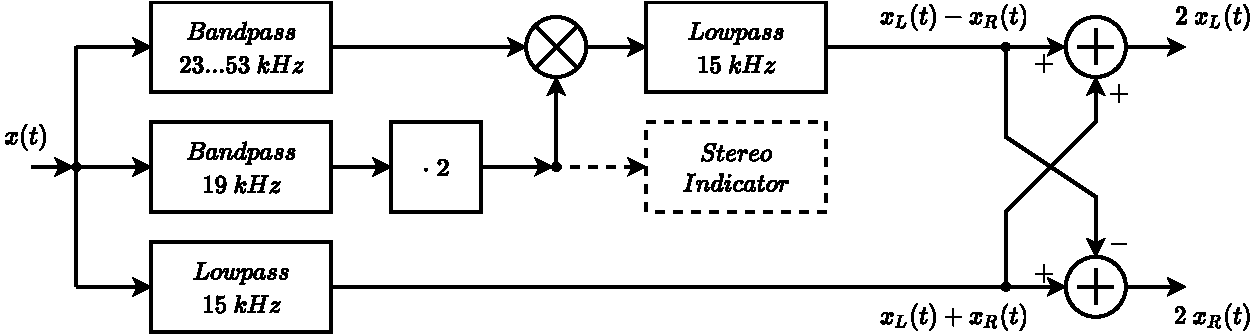
\includegraphics[width=1.0\textwidth]{img/draw.io/bd_fm_demod_stereo_audio}
  \caption{Block diagram of FM stereo audio demodulation \cite{RoppelBegleitmaterial}.}
  \label{fig_bd_stereo_demod}
\end{figure}

The central branch selects the pilot tone at 19 kHz with a bandpass filter.
This bandpass needs to have a frequency response that is sharp enough to have a sufficient attenuation at $\pm$4 kHz, since this is where the mono and difference signals' frequency spectra are allocated.
Afterwards, the pilot tone frequency is doubled to achieve a 38 kHz subcarrier.
This guarantees a phase-coherency between pilot and subcarrier, which is required to correctly shift the difference signal down to baseband.

The frequency doubling can be implemented with multiple methods.
The pilot tone can be modulated by simply multiplying it with itself.
Another option is to use a PLL and configure it to generate the double frequency at its output.
The PLL lock indicator can then be re-used as an indicator, whether a pilot tone is existent.\\

In the upper branch, a bandpass filter selects the difference signal with ranges from 23 to 53 kHz.
It is then modulated to baseband by the previously generated 38 kHz subcarrier.
Subsequently, a lowpass limits signal bandwidth to 15 kHz, which removes the generated modulation artifacts.\\

The lower branch lowpass-filters the summation, or mono signal, as described in paragraph \ref{subsec:demod_mono}.\\

The rightmost part in the diagram performs the combination of the mono and the difference signal, according to Eq.\eqref{equ_stereo_from_sum_diff}.
